\documentclass[10pt,a4paper]{article} 
% Style
\usepackage{amsfonts}
\usepackage{amsmath}
\usepackage{amssymb}
\usepackage[utf8]{inputenc}
\usepackage[T1]{fontenc}
\usepackage[swedish]{babel}
\usepackage{lmodern} 
\usepackage{graphicx}
\usepackage{color}
\usepackage{float}
\usepackage{listings}
\lstset{extendedchars=\true}
\lstset{inputencoding=ansinew}
\usepackage{hyperref}

% New commands
\newcommand{\degree}{\ensuremath{^\circ}}

% Formler

% Sources

% ---Title page ---

\title{Företagsanalys Tekniska verken}

\author{Johan Berneland, johbe915\\Sofia Larsson Cahlin, sofla266\\Benjamin Lundahl, benlu392\\
    Nora Björklund, norbj648\\Christopher Hallberg, chrha007}
\date{\today}

% ---Dokument start---

\begin{document}


\maketitle

\newpage

\tableofcontents

\newpage

\section{Inledning}
Denna rapport är en del i kursen Industriell ekonomi grundkurs, TEAE01, vid
Linköpings Universitet och utgörs av en analys av företaget Tekniska verken
i Linköping AB, org. nr: 556004-9727 (Retriever, 2013a).

\subsection{Bakgrund och syfte}
Syftet med denna rapport är att analysera om det valda företaget, Tekniska verken i Linköping AB, är en bra arbetsgivare. Detta sker genom att bedöma företaget främst utifrån de ekonomiska redskap och analysmetoder som getts inom ramarna för kursen. 
\subsection{Definition av bra arbetsgivare}
Vad som är en bra arbetsgivare är högst individuellt. För att kunna utföra analysen och dra slutsatser kring detta definieras här vilka aspekter som i denna rapport kännetecknar en bra arbetsgivare.

\begin{itemize}
 \item En säker anställningssituation, främst genom en stabil företagsekonomi 
 \item Bra företagsklimat
 \item Potential till personlig utveckling
 \item Marknadsanpassad ersättning
 \item Bra rykte och anseende
\end{itemize}

\section{Metod}
Rapporten grundar sig på data hämtad från årsredovisningar från företaget vad
gäller de ekonomiska delarna. I de delar som rör företagets historia, vision,
mission och liknande har vi använt oss av information från företagets hemsida.

\section{Resultat och analys}
Resultat och analys är uppdelad i tre olika avsnitt; först en beskrivning av
företaget, följt av en ekonomisk beskrivning och slutligen en SWOT-analys.

\subsection{Företagsbeskrivning}
För att kunna göra en korrekt analys av ett företag så behöver man veta vissa
grundförutsättningar. I följande avsnitt avhandlas några viktiga punkter. 

\subsubsection{Historia}
Grunden för Tekniska verken lades den 18 oktober 1902 genom startandet av
Linköpings elektriska kraft- och belysningsaktiebolag. Initiativtagare var en
entreprenör vid namn Jonn O Nilson och målet var att förse Linköpingsborna med
elström. År 1952 påbörjades fjärrvärmeutbyggnaden i Linköping och 2 år senare
kunde ett kraftvärmeverk leverera den första fjärrvärmen i Åbylund. Utbyggnaden
fortsatte och ytterligare kraftverk kom till under kommande årtionden. År 1981 
invigdes Gärstadsverket som utnyttjade avfall som bränsle. I samband med detta
började även utvecklingen för att ta till vara på avfall för att producera biogas 
och biogödsel. (Tekniska verken, 2013a) 

\subsubsection{Vision, mission, affärsidé}
Tekniska verkens vision är att ''bygga världens mest resurseffektiva
region'' och deras mission är ''att tillhandahålla och utveckla
ledningsbunden infrastruktur och energilösningar för den
resurseffektiva regionen'' (Tekniska Verken, 2013b). Det framgår även
från texter på deras hemsida att deras affärsidé är [FIXME].

\subsubsection{Ägarsituation och aktier}
Tekniska verken ägs av Linköping kommun (Tekniska verken, 2013c). Deras
aktiekapital uppgår i 200 miljoner kronor och det finns 400 tusen
aktier (Retriever, 2013a).

\subsubsection{Produkter och tjänster} \label{subsec:prod}
Tekniska verken erbjuder många tjänster inom många olika sektorer i samhället.
\begin{itemize}
	\item \textbf{Energi ur avfall:} Genom att sammla in brännbart avfall som energikälla kan fjärrvärme, fjärrkyla och el produceras till det nordiska elnätet. Dessutom i ackord med detta återvinner, behandlar och deponerar man avfall från hushåll
	och industrier.
	\item \textbf{Vatten:} Tkniska verken renar vatten från olika naturliga källor till
	dricksvatten. Dessutom behandlar och renar man avloppsvatten innan det släpps ut i naturen igen. Förutom det sammlar man samlar upp nederbörd och kvalitetstestar vatten i laboratorium.
	\item \textbf{Infrastruktur:} Tekniska verken driftum AB är en sammarbetspartner
	som tillsammans med Tekniska verken levererar konsulttjänster. Man fokuserar på områdena infrastruktur,
	mätteknik och energieffektivisering.
	\item \textbf{Nät:} Dotterbolaget Tekniska verken Linköping nät AB lägger fokus på nät och distribuerar regionalt elektricitet och bredband samt
	helhetslösningar för utomhusbelysning.
	\item \textbf{Bredband:} Tekniska verken är även delägare i bolaget Utsikt
	Bredband som levererar bredband till hushåll, företag, operatörer och fastighetsägare.
	\item \textbf{Miljövänlig el:} Tekniska verken är även delägare i bolaget Bixia
	AB, som köper in miljövänlig el från förnybara källor.
	\item \textbf{Biogas:} Dotterbolaget Svensk Biogas driver utvecklingen av
	marknaden för biogas och arbetar med etablering av tankställen för allmänheten.
	Dessutom utvecklar man processer och produktionskoncept.
	\item \textbf{Forskning och utveckling:} Tekniska verken arbetar även med att
	förbättra och utveckla processer som gynnar miljön och ekonomin.
\end{itemize}

(Tekniska verken, 2013d)
[dessutom vore det bra att skriva om detta stycke lite mer. Som det ser ut nu skulle det nog inte gå igenom urkund]

\subsubsection{Marknadsstrategi och kritiska framgångsfaktorer} \label{subsec:kff}
Tekniska verken marknadsför sig som föregångare inom miljövänlig teknik och
effektiva energilösningar. De vill framstå som en stor och trovärdig leverantör 
av många tjänster och tekniska lösningar, som nämnts i avsnitt \ref{subsec:prod}. 

En mycket trolig framgångsfaktor för Tekniska verken är det nära samarbetet med
kommunen. I flera sektorer har man genom sina uppdrag från kommunen i princip
monopol. Detta kan även ha haft positiv effekt när de etablerat sig i nya
sektorer då potentiella kunder ser dem som ett trovärdigt alternativ. 

Tekniska verkens profilering inom miljöområdet är en annan framgångsfaktor. Den
bidrar till en positiv image i mångas ögon. De har tagit en ``smutsig`` bransch
som avfallsindustrin, tidigare i princip ett nödvändigt ont, och inte bara tjänat 
pengar på den, utan också lyckats utvinna nytta.

\subsubsection{Marknader och marknadsandelar}
Tekniska verken är aktiva på flera olika marknader. Dessa presenteras nedan.\\

El och vatten: Den totala elanvändningen i Sverige 2012 uppgick till 131,9 TWh (SCB, 2012a). Av detta sålde Tekniska verken 5,4 TWh (Tekniska verken, 2013c) dvs ca 4 \% av den totala elanvändningen. Dessutom tillhandahåller de elnät  till ca 90 000 kunder i Linköping och Mjölby (Tekniska verken, 2013c), av totalt 68 795 (2011-12-31) (Linköpings kommun, 2013) respektive 11 763 (SCB, 2013) hushåll plus företag. År 2012 sålde de 12 miljoner kubikmeter vatten. \\

Värme och kyla: Den totala leveransen av fjärrvärme i Sverige 2012 uppgick till 52,3 TWh (SCB, 2012b). Av denna levererade Tekniska verken 1,547 TWh (Tekniska verken, 2013c) dvs de står för nästan 3\% av Sveriges fjärrvärmeleveranser. I och med att fjärrvärmen är starkt infrastrukturbunden kan det vara mer intressant att se till marknadsandelarna lokalt. 2012 levererade Tekniska verken fjärrvärme till 12 157 st (Tekniska verken, 2013c) av Linköpings 68 795 (2011-12-31) hushåll (Linköpings kommun, 2013) och 6 738 företagsförekomster (SCB, 2012b) dvs till ca 16 \% av de potentiella kunderna.\\

Bredband: År 2012 levererade Tekniska verken bredband till 12 500 privatkunder men de levererar även bredband till företag. Bredbandskunderna finns i  Linköping, Katrineholm och Mjölby. (Tekniska verken, 2013c)\\

Avlopp: Tekniska verken hade 2012 19 931 kunder för vatten och avlopp (Tekniska verken, 2013c) dvs ca 26 \% av alla hushåll och företag i Linköping enligt ovan. \\

Avfall: Tekniska verken hade 2012 17 660 kunder för avfall (Tekniska verken, 2013c) dvs ca 23 \% av alla hushåll och företag i Linköping enligt ovan. 

\subsubsection{Organisation}
Tekniska verken ägs av Linköpings kommun och ligger under Linköpings stadshus AB (Retriever, 2013a). Moderbolaget heter Tekniska verken i Linköping AB och har i sin tur åtta dotterbolag, främst med säten i Linköping men även i Katrineholm (Tekniska verken, 2013c).  Bolagets firma tecknas av en styrelse med nio stycken ordinarie ledamöter och nio suppleanter. Den verkställande ledningen utgörs av en ledningsgrupp bestående av vd och koncernchef Anders Jonsson, vice vd, finansdirektör och olika vd:ar och chefer för vissa dotterbolag. (Tekniska verken 2013b)

Företaget hade 969 anställda 2012 (Tekniska verken, 2013c; Retriever, 2013a) och i sin interna MMI-undersökning (Motiverad Medarbetar Index) från 2012 fick de 4,01 av 5 (Tekniska verken, 2013e). I FöretagsBarometern 2013 finns de också med på en lista över Sveriges mest attraktiva arbetsgivare för civilingenjörer (Tekniska verken, 2013f; Framtidsföretagen, 2013). 

\subsubsection{Omvärldsanalys, bransch, konkurrenter och intressenter}
Delar av tekniska verkens verksamhetsområden ligger i områden som inte
påverkas av konjunkturen i så hög grad. Det syns till exempel på
rörelseresultat och vinstmarginal som inte påverkats märkvärt mellan
2007 och 2012 under vilket Sverige genomlevde lågkonjunktur (Retriever, 2013; Konj, 2013). Detta beror på att verksamheterna, till exempel vattenrening och sopsorteringen, är lokala tjänster som används av 
invånarna i Linköpings samt omgivande kommuner och är en viktig del av 'kretsloppet' i kommunen.
Samtidigt så påverkas exempelvis elförsäljningen i hög grad av konjunkturen i
och med industrin.

Tekniska verken påverkas även kraftigt av klimatfaktorer som väderförhållanden 
som varierar under säsongerna och globala variationer i elpriser (Retriever, 2013a).

Eftersom Tekniska verken är delägare i många mindre bolag finns ingen enhetlig 
bransch, utan istället många olika branscher. Företaget är på så vis verksam inom
avloppshantering, sophantering, elhandel, elproduktion, fjärrvärme, fjärrkyla, 
nätverk och bredband. Man har alltså ett mycket brett spektrum vad gäller 
verksamhetsområdet. (Tekniska verken, 2013d)

De viktigaste intressenterna i Tekniska verken är ägaren, Linköpings kommun,
med dess invånare och företag. Tekniska verken är ansvariga för en rad tjänster
för kommuninvånarna, så som vatten och avlopp, avfallshantering, fjärrvärme och
elnät med mera. Vidare så är många invånare kunder till något av Tekniska
verkens dotterbolag. Exempelvis så är Bixia AB en stor el-leverantör och många
får sitt bredband genom Utsikt bredband ABs nät (Retriever, 2013a). 

Intressenter finns även utanför kommungränserna. Cirka 25 andra kommuner
levererar avfall till Gärstad (Tekniska verken, 2013g).

\subsubsection{Specifika uppförandekoder och spelregler} 
Då tekniska verken arbetar i många olika branscher, måste de även ha koll på
vilka regler som gäller inom alla dessa.

För avfallshantering måste man uppfylla de krav som ställs av Naturvårdsverket och
som innefattar EU:s avfallsdirektiv. [KÄLLA]

För produktion av dricksvatten måste man uppfylla de krav som ställs av Riksdag
och regeringen, Livsmedelsverket, Naturvårdsverket, Havs- och Vattenmyndigheten,
Socialstyrelsen, Boverket, Kemikalieinspektionen (KemI), Strålsäkerhetsmyndigheten 
(SSM) och EU:s lagstiftning. [KÄLLA]

För distribuering och marknadsföring av energi i olika former så som el och
fjärrvärme, måste man rikta sig efter de krav och regler som
energimarknadsinspektionen ställer. [KÄLLA]

\subsection{Social Beskrivning}
Då Tekniska Verken har en bred verksamhet så har de också ett brett
behov av anställda inom olika yrkesområden. Av dessa är en stor andel
anslutna till fackförbunden Kommunal och Vision (Jacobsson S,
2013). Det erbjuds möjligheter att avancera inom bolaget till exempel
genom ledarskapsutbildningar finansierade av Tekniska Verken
(Jacobsson S, 2013). 

En kontrovers inom företaget skulle vara lönerna för hög- och
lågavlönade. Det framgår i en artikel publicerad i Kommunal Arbetaren samt i ett
debattinlägg i Corren att lönerna för bland annat anläggningsarbetare
och fordonsförare ligger under de marknadsmässiga lönerna (KA, 2012;
Corren, 2008). Detta medan debatt har skapats kring att bland annat
verkställande direktör för Tekniska Verken är väldigt hög för att vara
en kommunal chef (Corren, 2013).

Ungefär en tredjedel av de anställda på Tekniska Verken är
kvinnor. Dock sitter det bara en kvinna i bolagets ledning
(Tekniska Verken, ). Tekniska Verken är en historiskt sett mansdominerad bransch
men har haft ett ökande antal kvinnor som söker och får jobb
(Jacobsson S, 2013).  
\subsection{Ekonomisk beskrivning}
Syftet med följande avsnitt är att få en inblick i Tekniska verkens ekonomiska
situation.

\subsubsection{Nyckeltal}
Vi har plockat ut de nyckeltal vi anser mest relevanta med tanke på vårat syfte och listat dem i tabell \ref{table:nyckeltal}. Överlag har de utvalda nyckeltalen med anställda eller företagets ekonomiska stabilitet att göra.

Inga nyckeltal skiljer sig nämnvärt från de intervall tumreglerna som tagits upp i kursen föreslår.
\begin{table}[h]
	\begin{tabular}{ l r }
		antal anställda, aktiebolag & 969\\
		löner till övr. anställda & 387 883\\
		avkastning på eget kapital (\%) & 14,16\\
	%%	avkastning på totalt kapital (\%) & 6,85\\
	%%	skuldränta (\%) & 2,19\\
	%%	riskbuffert totalt kapital & 4,66\\
	%%	rörelseresultat före avskrivningar, ebitda & 1 052 000\\
	%%	rörelsemarginal (\%) & 10,64\\
		vinstmarginal (\%) & 10,89\\
		omsättning per anställd & 5 410,73\\
		soliditet (\%) & 39,39\\
	%%	kapitalets omsättningshastighet & 0,63\\
	%%	rörelsekapital & 957 000\\
	%%	rörelsekapital/omsättning (\%) & 18,25\\
		kassalikviditet (\%) & 159\\
		förändring av omsättning (\%) & -7,27\\
	%%	rörelseresultat per anställd & 575,85\\
		personalkostnader per anställd & 631,58\\
		förändring av antal anställda (\%) & -0,31\\
	%%	lager mm/omsättning (\%) & 2,25\\
	%%	kundfordringar/omsättning (\%) & 10,41\\
	%%	likvida medel/omsättning (\%) & 11,81\\
	%%	kortfristiga skulder/omsättning (\%) & 27,12\\
	%%	skuldsättningsgrad (\%) & 1,48\\
	%%	räntetäckningsgrad (\%) & 5,39\\
	%%	avkastning operativt kapital (\%) & 8,86\\
	%%	riskbuffert sysselsatt kapital st & 5,29\\
	%%	varulagrets omsättningshastighet & 0\\
	%%	du pont-modellen (\%) & 6,85\\

	\end{tabular}
	\caption{nyckeltal avseende 2012, siffror i tusentals kronor om annat ej anges. (Retriever 2013a)}
	\label{table:nyckeltal}
\end{table}

\subsubsection{Jämförelse över tid} 
Som kan ses i figur \ref{fig:jamfor} har Tekniska verkens nyckeltal legat
förhållandevis konstanta under de senaste åren. Man kan se en stadigt ökande trend vad gäller soliditeten medan antalet anställda fluktuerat något, men ökat över tid. (Retriever, 2013a)
\begin{figure}[H] 
\centerline{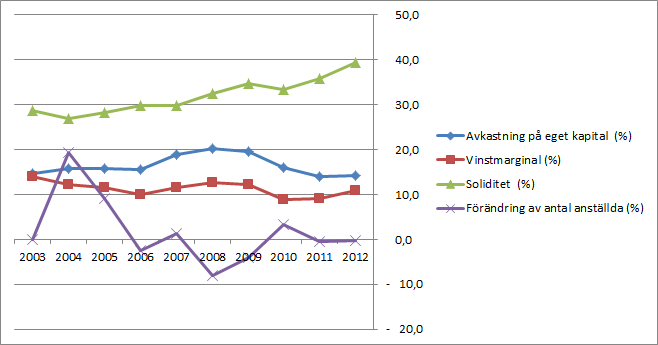
\includegraphics[scale=0.8]{Bilder/jamforelse_over_tid.png}}
\caption{Jämförelse över tid. (Retriever, 2013a)}
\label{fig:jamfor}
\end{figure}  

\subsubsection{Jämförelse med konkurrenter}
Vid jämförelse med två likartade företag inom samma bransch, Göteborg energi och Fortum värme samägt med Stockholms stad, kan man se att alla tre går ganska jämnt. Tekniska verken har en något högre avkastning på eget kapital än de andra två. De har dessutom ökat sin likviditet över den senaste 5-års perioden, medan Fortum har legat stabilt och Göteborg energi har minskat. (Retriever, 2013b; Retriever, 2013c)
\subsection{SWOT-analys}
Nedan presentera en SWOT-analys för Tekniska verken, dvs en analys för företagets nuläge genom styrkor och svagheter men även potentiella framtida hot och möjligheter. 

\subsubsection{Styrkor (Strengths)}
I avsnittet om kritiska framgångsfaktorer, \ref{subsec:kff}, nämndes ett antal
saker som kan ses som styrkor, exempelvis samarbetet med kommunen och
miljöinriktningen. Andra styrkor är företagets storlek och det
faktum att man arbetar i många branscher som är mindre känsliga för det
ekonomiska läget än andra industriföretag. Tittar man på de ekonomiska
nyckeltalen och jämförelsen över tiden så pekar de på god stabilitet och bra
resultat. Ur anställningssynpunkt ter sig Tekniska verken som en relativt 
stabil arbetsgivare i den mening att inga större uppsägningar skett på senare
år, som kan ses i tabell \ref{table:nyckeltal}. Krisåret 2008 skulle möjligtvis
kunna ses som ett undantag även om det inte rör sig om en stor förändring.

\subsubsection{Svagheter (Weaknesses)}
\begin{itemize}
	\item \textbf{Infrastruktursberoende:}
		Förmågan att utvidga kundbasen inom bredband, fjärrvärme, elnät, vatten och avlopp och biogas är direkt beroende av en kostsam infrastruktur som tar tid att bygga. Detta gör att Tekniska verken får det svårare att expandera till andra städer inom dessa områden. När det gäller fjärrvärme exemplifieras detta i figur \ref{fig:fjarr}.
		
\end{itemize}
\begin{figure}[H] 
\centerline{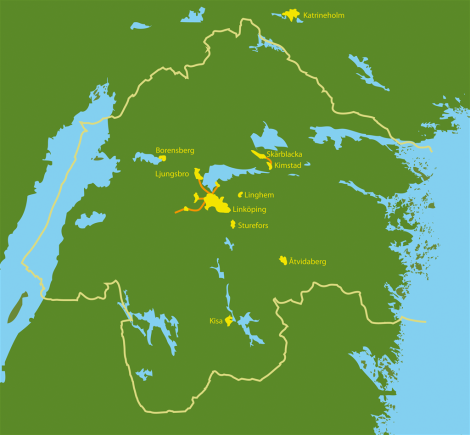
\includegraphics[scale=0.5]{Bilder/teckning_fjarrvarme.png}}
\caption{Täckning av fjärrvärme i Östergötland med omnejd (gulmarkerat) (Tekniska verken, 2013h)}
\label{fig:fjarr}
\end{figure}  


\subsubsection{Möjligheter (Opportunities)}
Möjligheterna för ett företag som tekniska verken är många då man har verksamhet i så många olika grenar. 

En stor framtida möjlighet är inom produktion av vätgas eller vätgasbärande vätskor. Vätgas går både att använda i förbränningsmotorer, likt de som redan existerar i dagens bilar och i så kallade bränslecellsdrivna bilar. 

Den största utmaningen med vätgas är just lagringen eftersom gasen antänder mycket lätt. Det forskas mycket om att försöka använda metaller eller andra ämnen för att kunna lagra vätgasen på ett säkert sätt med minimala energiförluster.

\begin{figure}[H] 
\centerline{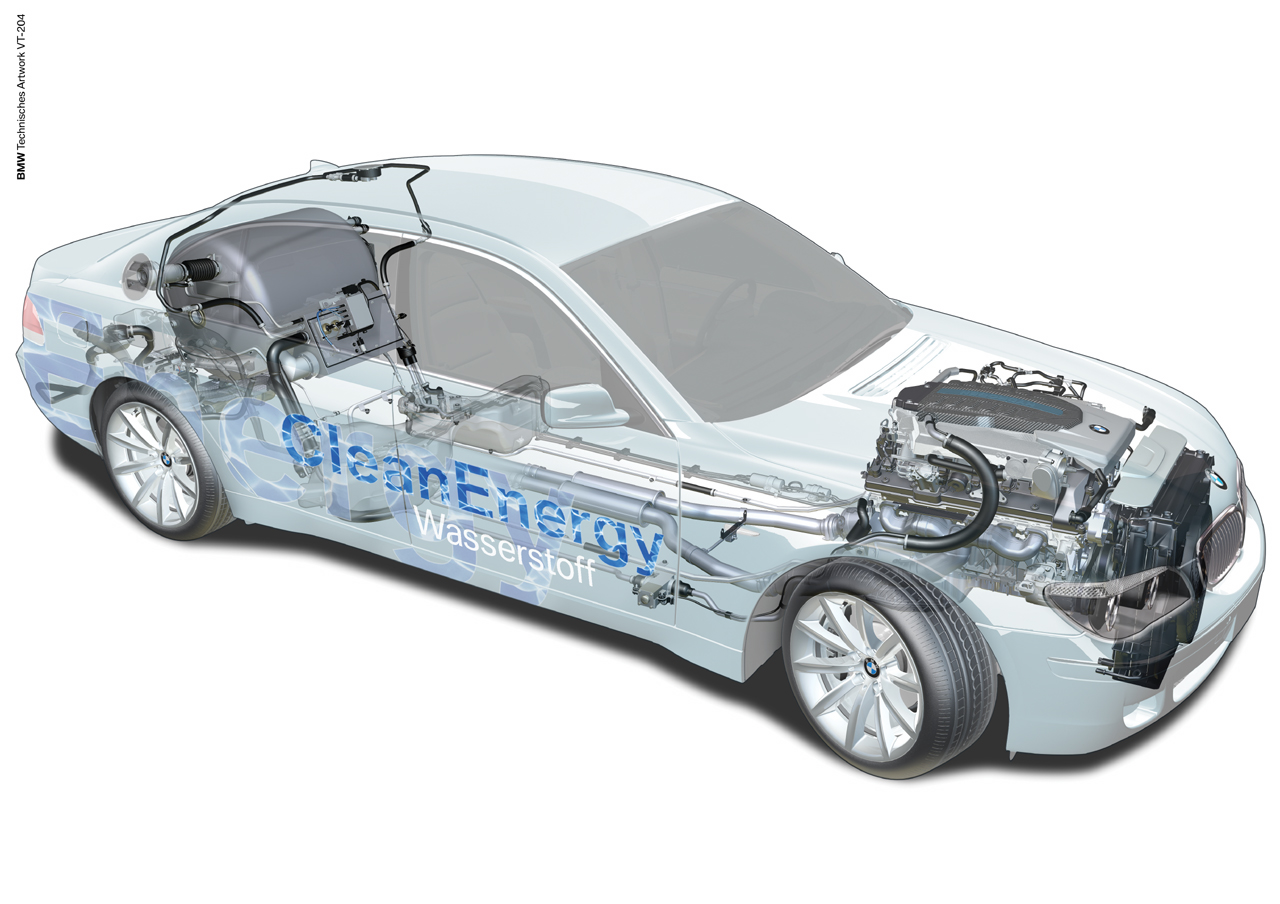
\includegraphics[scale=0.14]{Bilder/bmwcar.jpg}}
\caption{BMW 7 series med 12 cylinder motor som kan använda både vätgas så som bensin som bränsle.}
\label{fig:bmw}
\end{figure}

%%Utökning av infrastruktur

\subsubsection{Hot (Threats)}
Det som skulle kunna ses som ett större hot mot Tekniska Verken är
att någon av deras större investeringar misslyckas eller
utkonkurreras. Koncernen Tekniska Verken sköter stora tekniska system som är
kostsamma att bygga upp men också är en del av
samhällsfunktionen. Några av dessa är kommunala monopol och
verksamheter som bara Tekniska Verken kan och får sköta.(Jacobsson S, 2013) 

Ett annat hot mot Tekniska Verken skulle alltså kunna vara om monopolet
skulle sluta gälla och fler aktörer släpptes in, eller att kommunen
skulle lägga uppdraget på en annan aktör. Med tanke på Tekniska Verkens förrankring i kommunen
och goda resultat så är riskerna för att kommunen skulle lägga ner
bolaget, eller delar av det mycket liten. Diskussioner bland
intresseorganisationer har pågått om
monopolet på fjärrvärme bör skrotas, men även om det gör det har
Tekniska Verken en enorm fördel genom att redan vara etablerad aktör
(NyTeknik, 2013a; NyTeknik, 2013b).

\section{Slutsatser}
I följande kapitel följer våra slutsatser utifrån det som diskuterats tidigare i
arbetet. Enligt tidigare definition kännetecknas en bra arbetsgivare av att 
följande kriterier är uppfyllda.

\begin{itemize}
 \item En säker anställningssituation, främst genom en stabil företagsekonomi 
 \item Bra företagsklimat
 \item Potential till personlig utveckling
 \item Marknadsanpassad ersättning
 \item Bra rykte och anseende
\end{itemize}

Antalet anställda vid Tekniska verken har legat stabilt de senaste åren. Likaså
visar övriga ekonomiska nyckeltal, enligt vår analys, på en stabil
företagsekonomi med god tillväxt.

Tekniska verken tycks ha bra rykte och anseende. Profileringen inom miljöområdet
ger ett positivt intryck och allt tyder på att de generellt är ansedda som ett
pålitligt företag. Vi har inte lyckats hitta något som tyder på att deras rykte
eller anseende av någon anledning skulle kunna ses som negativt.

\newpage
\section{Referenser}
%% Här placeras referenser enligt Harvard metoden. Skall vara alfabetiskt, för
%% övrig info se harvard-lathunden.
%%


\hspace{0,5cm}Energimarknadsinspektionen, (2013). Avfallshantering. (HTML) Tillgänglig: \\
\hyperref{http://www.energimarknadsinspektionen.se/sv/el/}{}{}{http://www.energimarknadsinspektionen.se/sv/el/(2013-11-20)}\\

Framtidsföretagen, (2013). Utmanare civilingenjör. (HTML) Tillgänglig: \\
http://www.framtidsforetagen.se/rankings/utmanare-civilingenjor/ (2013-12-11)\\

Jacobsson, S. (2013), Marknadsdirektör Tekniska Verken AB, Frågor om
Tekniska Verkens Nuläge.\\
Telefon intervju gjord av Nora Björklund. Datum: 2013-12-13. \\

Konj, (2013). Konjunkturläget juni 2013. (PDF) Tillgänglig:\\
\hyperref{http://www.konj.se/download/18.6a90e2ce13e070b080d1a1f/Konjunkturl\%C3\%A4get+juni+2013.pdf}{}{}{<http://www.konj.se/download/18.6a90e2ce13e070b080d1a1f/Konjunkturl\%C\\3\%A4get+juni+2013.pdf> (2013-12-04)}\\

Linköpings kommun, (2013). Hushåll. (PDF) Tillgänglig:\\
http://www.linkoping.se/Global/Om\%20kommunen/Fakta\%20om\%20Linköping/\\Statistiska\%20fakta\%20om\%20Linköping/Kortfakta/hushall.pdf (2013-12-11)\\

Naturvårdsverket, (2013). Avfallshantering. (HTML) Tillgänglig: \\
\hyperref{http://www.naturvardsverket.se/Stod-i-miljoarbetet/Vagledning-amnesvis/Avfall/Lagar-och-regler-om-avfall/}{}{}{http://www.naturvardsverket.se/Stod-i-miljoarbetet/Vagledning-amnesvis/Avfall/Lagar-och-regler-om-avfall/(2013-11-20)}\\
NyTeknik, (2013a). Gärna konkurrens men på lika villkor. (HTML)
Tillgänglig: \\
\hyperref{http://www.nyteknik.se/asikter/debatt/article3777742.ece}{}{}{<http://www.nyteknik.se/asikter/debatt/article3777742.ece>
  (2013-12-13)}\\

NyTeknik, (2013b). Skrota monopolet på fjärrvärme. (HTML)
Tillgänglig: \\
\hyperref{http://www.nyteknik.se/asikter/debatt/article3774196.ece}{}{}{<http://www.nyteknik.se/asikter/debatt/article3774196.ece>
  (2013-12-13)}\\

Retriever, (2013a). AB Fortum Värme samägt med Stockholms stad (HTML) Tillgänglig: \\
http://web.retriever-info.com/services/\\businessinfo.html?method=displayBusinessInfo\&orgnum=5560169095\\(2013-12-13)\\

Retriever, (2013b). Göteborg energi AB. (HTML) Tillgänglig: \\
http://web.retriever-info.com/services/\\businessinfo.html?method=displayBusinessInfo\&orgnum=5563626794\\
(2013-12-13)\\

Retriever, (2013c). Tekniska verken i Linköping AB. (HTML) Tillgänglig: \\
\hyperref{http://web.retriever-info.com/services/businessinfo.html?method=displayBusinessInfo\&orgnum=5560049727}{}{}{<http://web.retriever-info.com/services/businessinfo.html?method=displayBu\\sinessInfo\&orgnum=5560049727> (2013-12-04)}\\

SCB, (2012a). El-, gas- och fjärrvärmeförsörjningen 2012. (PDF) Tillgänglig:\\
http://www.scb.se/Statistik/EN/EN0105/2012A01/EN0105\_2012A01\_SM\_EN11SM1302.pdf (2013-12-11)\\

SCB, (2012b). Registerbaserad arbetsmarknadsstatistik (RAMS) (PDF) Tillgänglig:\\
http://www.scb.se/sv\_/Hitta-statistik/Statistik-efter-amne/Arbetsmarknad/ \\Sysselsattning-forvarvsarbete-och-arbetstider/Registerbaserad-arbetsmarknadsstatistik-RAMS/7895/7902/117037/ (2013-12-11)\\

SCB, (2013). Statistikdatabasen 2013. (HTML) Tillgänglig:\\
http://www.scb.se/sv\_/Hitta-statistik/Statistikdatabasen/TabellPresentation/?\\layout=tableViewLayout1\&rxid=5b78f422-ba93-40a7-a2c2-d4ede68cba62 (2013-12-11)\\

Svenskt Vatten, (2013). Dricksvatten. (HTML) Tillgänglig: \\
\hyperref{http://www.svensktvatten.se/Vattentjanster/Dricksvatten/Lagar-och-foreskrifter/}{}{}{<http://www.svensktvatten.se/Vattentjanster/Dricksvatten/Lagar-och-foreskrifter/>
(2013-11-20)} \\

Tekniska verken, (2013a). Historiska boken. (PDF) Tillgänglig: \\
\hyperref{http://www.tekniskaverken.se/om-oss/var-historia/historiska-boken/}{}{}{<http://www.tekniskaverken.se/om-oss/var-historia/historiska-boken/> (2013-11-20)}\\

Tekniska verken, (2013b). Ledning. (HTML) Tillgänglig: \\
http://www.tekniskaverken.se/om-oss/ekonomiorganisation/ledning/ (2013-12-11)\\

Tekniska verken, (2013c). Kortfakta. (HTML) Tillgänglig: \\
http://www.tekniskaverken.se/om-oss/ekonomiorganisation/kortfakta/ (2013-12-11)\\

Tekniska verken, (2013d). Tjänster. (HTML) Tillgänglig: \\
\hyperref{http://www.tekniskaverken.se/tjanster/}{}{}{<http://www.tekniskaverken.se/tjanster/>
  (2013-11-20)}\\

Tekniska verken, (2013e). Medarbetarnöjdhet. (HTML) Tillgänglig: \\
https://www.tekniskaverken.se/om-oss/jobb/medarbetare/medarbetarnojdhet/ (2013-12-11)\\

Tekniska verken, (2013f). Jobb. (HTML) Tillgänglig: \\
https://www.tekniskaverken.se/om-oss/jobb/ (2013-12-11)\\

Tekniska verken, (2013g). Avfall \& återvinning. (HTML) Tillgänglig: \\
\hyperref{http://www.tekniskaverken.se/avfall-atervinning/om/}{}{}{<http://www.tekniskaverken.se/avfall-atervinning/om/> (2013-11-27)} \\

Tekniska verken, (2013h). Kan jag få fjärrvärme? (HTML) Tillgänglig:\\ 
http://www.tekniskaverken.se/komfort/privat/jag-ar-intresserad-av-fja/\\kan-jag-fa-fjarrvarme/ (2013-12-13)

BMW, (2013). Möjligheter. (HTML) Tillgänglig: \\
\hyperref{http://www.bmw.com/com/en/insights/technology/efficient_dynamics/phase_2/clean_energy/bmw_hydrogen_7.html}{}{}{<http://www.bmw.com/com/en/insights/technology/efficient\_dynamics/\\phase\_2/clean\_energy/bmw\_hydrogen\_7.html>(2013-12-13)}\\

Vätgas lagring, (2013). Möjligheter. (HTML) Tillgänglig: \\
\hyperref{http://www.hydrogen.energy.gov/storage.html}{}{}{<http://www.hydrogen.energy.gov/storage.html>(2013-12-13)}\\

\end{document}



%%% Local Variables: 
%%% TeX-PDF-mode: t 
%%% TeX-master: "rapport"
%%% End: 

